\section{Faster matrix multiplication: Full results}

\paragraph{Full table of results.} We provide the best ranks obtained by \method in~\Cref{tab:relaxed-opt-results-appendix}. Overall, we considered 54 matrix multiplication sizes in our experiments. These were chosen roughly representing sizes $\langle m,n,p \rangle$ where $2\leq m,n\leq 5$, with some reasonable cutoff for $p$. Due to symmetries of the underlying matrix multiplication tensor, there exist equivalent algorithms for any permutations of the three axes, hence we focus on sorted sizes $m\leq n\leq p$.

In all but two considered sizes, \method discovered programs which either match or surpass the best known rank. Anecdotally, we encountered some difficulty when increasing the problem size: when we run the discovered programs on sizes beyond $\langle 5,5,5 \rangle$ on 1000 random seeds on evaluators with a single GPU accelerator, we often run out of memory. Hence, extending our setup to larger matrix sizes requires further optimization.

\begin{table}[h]
\rowcolors{2}{white}{gray!30}
\begin{center}
    \scalebox{0.7}{
    \begin{tabular}{ccc}
    $\langle m, n, p \rangle$ & \makecell{best known \\ {[reference]}}  & \method \\ \midrule
    $\langle 2, 2, 2 \rangle$ & 7 \citep{strassen1969gaussian}   & 7   \\ 
    $\langle 2, 2, 3 \rangle$ & 11~\citep{smirnov2013bilinear}& 11 \\ 
    $\langle 2, 2, 4 \rangle$ & 14~\citep{smirnov2013bilinear} & 14 \\ 
    $\langle 2, 2, 5 \rangle$ & 18~\citep{smirnov2013bilinear} & 18 \\ 
    $\langle 2, 2, 6 \rangle$ & 21~\citep{smirnov2013bilinear} & 21 \\ 
    $\langle 2, 2, 7 \rangle$ & 25~\citep{smirnov2013bilinear} & 25 \\ 
    $\langle 2, 2, 8 \rangle$ & 28~\citep{smirnov2013bilinear} & 28 \\ 
    $\langle 2, 2, 9 \rangle$ & 32~\citep{smirnov2013bilinear} & 32 \\ 
    $\langle 2, 2, 10 \rangle$ & 35~\citep{smirnov2013bilinear} & 35 \\ 
    $\langle 2, 2, 11 \rangle$ & 39~\citep{smirnov2013bilinear} & 39 \\ 
    $\langle 2, 2, 12 \rangle$ & 42~\citep{smirnov2013bilinear} & 42 \\ 
    $\langle 2, 2, 13 \rangle$ & 46~\citep{smirnov2013bilinear} & 46 \\ 
    $\langle 2, 2, 14 \rangle$ & 49~\citep{smirnov2013bilinear} & 49 \\ 
    $\langle 2, 2, 15 \rangle$ & 53~\citep{smirnov2013bilinear} & 53 \\ 
    $\langle 2, 2, 16 \rangle$ & 56~\citep{smirnov2013bilinear} & 56 \\ 
    $\langle 2, 3, 3 \rangle$ & 15~\citep{smirnov2013bilinear} & 15 \\ 
    $\langle 2, 3, 4 \rangle$ & 20~\citep{smirnov2013bilinear} & 20 \\ 
    $\langle 2, 3, 5 \rangle$ & 25~\citep{smirnov2013bilinear} & 25 \\ 
    \end{tabular}
    }
    \scalebox{0.7}{
    \begin{tabular}{ccc}
    $\langle m, n, p \rangle$ & \makecell{best known \\ {[reference]}}  & \method \\ \midrule
    $\langle 2, 3, 6 \rangle$ & 30~\citep{smirnov2013bilinear} & 30 \\ 
    $\langle 2, 3, 7 \rangle$ & 35~\citep{smirnov2013bilinear} & 35 \\ 
    $\langle 2, 3, 8 \rangle$ & 40~\citep{smirnov2013bilinear} & 40 \\ 
    $\langle 2, 3, 9 \rangle$ & 45~\citep{smirnov2013bilinear} & 45 \\ 
    $\langle 2, 3, 10 \rangle$ & 50~\citep{smirnov2013bilinear} & 50 \\ 
    $\langle 2, 4, 4 \rangle$ & 26~\citep{smirnov2013bilinear} & 26 \\ 
    $\langle 2, 4, 5 \rangle$ & 33~\citep{hopcroft} & \textcolor{darkgreen}{\textbf{32}} \\
    $\langle 2, 4, 6 \rangle$ & 39~\citep{smirnov2013bilinear} & 39 \\ 
    $\langle 2, 4, 7 \rangle$ & 46~\citep{smirnov2013bilinear} & \textcolor{darkgreen}{\textbf{45}} \\
    $\langle 2, 4, 8 \rangle$ & 52~\citep{smirnov2013bilinear} & \textcolor{darkgreen}{\textbf{51}} \\
    $\langle 2, 5, 5 \rangle$ & 40~\citep{smirnov2013bilinear} & 40 \\ 
    $\langle 2, 5, 6 \rangle$ & 48~\citep{smirnov2013bilinear} & \textcolor{darkgreen}{\textbf{47}} \\ 
    $\langle 3, 3, 3 \rangle$ & 23~\citep{laderman}   & 23   \\
    $\langle 3, 3, 4 \rangle$ & 29~\citep{smirnov2013bilinear} & 29 \\ 
    $\langle 3, 3, 5 \rangle$ & 36~\citep{smirnov2013bilinear} & 36 \\ 
    $\langle 3, 3, 6 \rangle$ & 40~\citep{smirnov2013bilinear} & 40 \\ 
    $\langle 3, 3, 7 \rangle$ & 49~\citep{smirnov2013bilinear} & 49 \\ 
    $\langle 3, 3, 8 \rangle$ & 55~\citep{smirnov2013bilinear} & 55 \\ 
    \end{tabular}
    }
    \scalebox{0.7}{
    \begin{tabular}{ccc}
    $\langle m, n, p \rangle$ & \makecell{best known \\ {[reference]}}  & \method \\ \midrule
    $\langle 3, 4, 4 \rangle$ & 38~\citep{smirnov2013bilinear} & 38 \\ 
    $\langle 3, 4, 5 \rangle$ & 47~\citep{fawzi2022discovering} & 47 \\ 
    $\langle 3, 4, 6 \rangle$ & 56~\citep{Kauers_2025} & \textcolor{darkgreen}{\textbf{54}} \\ 
    $\langle 3, 4, 7 \rangle$ & 66~\citep{smirnov2021} & \textcolor{darkgreen}{\textbf{63}} \\ 
    $\langle 3, 4, 8 \rangle$ & 75~\citep{smirnov2021}   & \textcolor{darkgreen}{\textbf{74}} \\ 
    $\langle 3, 5, 5 \rangle$ & 58~\citep{smirnov2021} & 58 \\ 
    $\langle 3, 5, 6 \rangle$ & 70~\citep{Kauers_2025} & \textcolor{darkgreen}{\textbf{68}} \\
    $\langle 3, 5, 7 \rangle$ & 82~\citep{smirnov2021} & \textcolor{darkgreen}{\textbf{80}} \\ 
    $\langle 4, 4, 4 \rangle$ & 49~\citep{strassen1969gaussian} & \textcolor{darkgreen}{\textbf{48}}  \\ 
    $\langle 4, 4, 5 \rangle$ & 62~\citep{kauers2023flip}   & \textcolor{darkgreen}{\textbf{61}}    \\
    $\langle 4, 4, 6 \rangle$ & 73~\citep{Kauers_2025} & 73 \\ 
    $\langle 4, 4, 7 \rangle$ & 87~\citep{smirnov2013bilinear,strassen1969gaussian} & \textcolor{darkgreen}{\textbf{85}}    \\
    $\langle 4, 4, 8 \rangle$ & 98~\citep{strassen1969gaussian} & \textcolor{darkgreen}{\textbf{96}} \\ 
    $\langle 4, 4, 9 \rangle$ & 104~\citep{smirnov2022} & \textcolor{purple}{108} \\ 
    $\langle 4, 5, 5 \rangle$ & 76~\citep{fawzi2022discovering} & 76 \\ 
    $\langle 4, 5, 6 \rangle$ & 93~\citep{Kauers_2025}   & \textcolor{darkgreen}{\textbf{90}} \\ 
    $\langle 5, 5, 5 \rangle$ & 93~\citep{flip_graphs_with_symmetry} & 93 \\ 
    $\langle 6, 6, 6 \rangle$ & 153~\citep{flip_graphs_with_symmetry} & \textcolor{purple}{156} \\ 
    \end{tabular}
    }
\caption{Full version of \Cref{tab:relaxed-opt-results}, showing the best ranks obtained by \method for tensor decomposition for all considered parameters. Of the 54 targets, \method matches the state of the art in 38 cases, surpasses it in 14 cases (green), and falls behind in 2 cases (red). In all cases, \method provides exact algorithms, using integer or half-integer entries in the decomposition. For $\langle 3, 4, 7\rangle$, $\langle 4, 4, 4\rangle$, and $\langle 4, 4, 8\rangle$, the algorithms discovered by \method use complex-valued multiplications which can be used for exact multiplication of complex or real-valued matrices. The decompositions shown in this table can be found in \ResultsColab.}
    \label{tab:relaxed-opt-results-appendix}
\end{center}
\end{table}

\emph{Note}: Concurrent work~\cite{kauers2025consequences} has also found a rank-$90$ algorithm for $\langle 4, 5, 6 \rangle$.

\paragraph{Magnified version of \Cref{fig:relaxed-opt-diff} (left).} In \Cref{fig:relaxed-opt-diff-appendix-1,fig:relaxed-opt-diff-appendix-2,fig:relaxed-opt-diff-appendix-3}, we show a magnified version of \Cref{fig:relaxed-opt-diff} (left), which corresponds to the program that discovers a decomposition of rank 48 for the 3D tensor representing the operation of multiplying two $4\times 4$ matrices. 

\begin{figure}[p]
\renewcommand{\thefigure}{\arabic{figure}a}\vspace{-0.03\textwidth}
\begin{adjustbox}{width=0.9\textwidth}
\begin{minipage}{0.9\textwidth}
\begin{lstlisting}[style=pydiff, backgroundcolor=\color{backcolour}]
@@ -45,9 +45,14 @@
   # EVOLVE-BLOCK-START
   def _get_optimizer(self) -> optax.GradientTransformation:
     """Returns optimizer."""
-    return optax.adam(self.hypers.learning_rate)
+    return optax.adamw(
+        self.hypers.learning_rate, weight_decay=self.hypers.weight_decay
+    )
 
   def _get_init_fn(self) -> jax.nn.initializers.Initializer:
     """Returns initializer function."""
-    return initializers.normal(0.0, self.hypers.init_scale, jnp.complex64)
+    # Initialize with a smaller scale to encourage finding low-rank solutions.
+    # Increase scale slightly for better exploration.
+    scale = self.hypers.init_scale
+    return initializers.normal(0 + 1j * 0, scale * 0.2, jnp.complex64)

@@ -80,6 +85,66 @@
     # Gradient updates.
     updates, opt_state = self.opt.update(grads, opt_state, decomposition)
     decomposition = optax.apply_updates(decomposition, updates)
+    # Add a small amount of gradient noise to help with exploration
+    rng, g_noise_rng = jax.random.split(rng)
+    decomposition = jax.tree_util.tree_map(
+        lambda x: x
+        + self.hypers.grad_noise_std * jax.random.normal(g_noise_rng, x.shape),
+        decomposition,
+    )
+
+    # Add noise to the decomposition parameters (exploration).
+    _, noise_rng = jax.random.split(rng)
+    noise_std = self._linear_schedule(
+        global_step, start=self.hypers.noise_std, end=0.0
+    )
+    decomposition = jax.tree_util.tree_map(
+        lambda x: x + noise_std * jax.random.normal(noise_rng, x.shape),
+        decomposition,
+    )
+
+    # Cyclical annealing for clipping threshold.
+    cycle_length = 2000  # Number of steps per cycle
+    cycle_progress = (
+        global_step % cycle_length
+    ) / cycle_length  # Normalized progress within the current cycle [0, 1)
+
+    # Map cycle progress to a sinusoidal curve. Ranges from 0 to 1.
+    clip_threshold_multiplier = (1 + jnp.cos(2 * jnp.pi * cycle_progress)) / 2
+
+    clip_threshold = self.hypers.clip_min + clip_threshold_multiplier * (
+        self.hypers.clip_max - self.hypers.clip_min
+    )
+
+    def soft_clip(x, threshold):
+      # Clipping the real and imaginary parts separately.
+      x_re = jnp.real(x)
+      x_im = jnp.imag(x)
+
+      x_re_clipped = jnp.where(
+          x_re > threshold, threshold + (x_re - threshold) * 0.1, x_re
+      )
+      x_re_clipped = jnp.where(
+          x_re_clipped < -threshold,
+          -threshold + (x_re_clipped + threshold) * 0.1,
+          x_re_clipped,
+      )
\end{lstlisting}
\end{minipage}
\end{adjustbox}
\caption{
Magnified version of~\Cref{fig:relaxed-opt-diff}(left), giving the program that discovers a faster algorithm to multiply $4\times4$ matrices (\emph{1/3}).}\label{fig:relaxed-opt-diff-appendix-1}
\centering
\end{figure}
\addtocounter{figure}{-1}


\begin{figure}[p]
\renewcommand{\thefigure}{\arabic{figure}b}\vspace{-0.03\textwidth}
\begin{adjustbox}{width=0.9\textwidth}
\begin{minipage}{0.9\textwidth}
\begin{lstlisting}[style=pydiff, backgroundcolor=\color{backcolour}, firstnumber=66]
+
+      x_im_clipped = jnp.where(
+          x_im > threshold, threshold + (x_im - threshold) * 0.1, x_im
+      )
+      x_im_clipped = jnp.where(
+          x_im_clipped < -threshold,
+          -threshold + (x_im_clipped + threshold) * 0.1,
+          x_im_clipped,
+      )
+
+      return x_re_clipped + 1j * x_im_clipped
+
+    decomposition = jax.tree_util.tree_map(
+        lambda x: soft_clip(x, clip_threshold), decomposition
+    )
+
     return decomposition, opt_state, loss
 
   def _loss_fn(
@@ -91,13 +156,86 @@
     """Computes (batched) loss on learned decomposition."""
     # Compute reconstruction loss.
     rec_tensor = self._decomposition_to_tensor(decomposition)  # (B, N, M, P)
+
+    # Add noise to the target tensor (robustness).
+    rng, noise_rng = jax.random.split(rng)
+    target_noise = self.hypers.target_noise_std * jax.random.normal(
+        noise_rng, self.target_tensor.shape
+    )
+    noisy_target_tensor = self.target_tensor + target_noise
+
+    # Hallucination loss (encourages exploration by randomly replacing values)
+    hallucination_prob = self.hypers.hallucination_prob
+    hallucination_scale = self.hypers.hallucination_scale
+
+    def hallucinate(x, hallucination_rng):
+      mask = jax.random.bernoulli(hallucination_rng, p=hallucination_prob)
+      noise = hallucination_scale * jax.random.normal(
+          hallucination_rng, x.shape
+      )
+      return jnp.where(mask, noise, x)
+
+    _, factor_rng = jax.random.split(rng)
+    decomposition = jax.tree_util.tree_map(
+        lambda x: hallucinate(x, jax.random.split(factor_rng)[0]),
+        decomposition,
+    )
+
     # Add a batch dimension to `target_tensor` to ensure correct broadcasting.
     # Define the loss as the L2 reconstruction error.
-    rec_loss = l2_loss_complex(self.target_tensor[None, ...], rec_tensor)
+    rec_loss = l2_loss_complex(noisy_target_tensor[None, ...], rec_tensor)
 
     # We must return a real-valued loss.
-    return jnp.real(rec_loss)
 
+    # Discretization loss (encourage entries to be multiples of 1/2 or integer).
+    def dist_to_half_ints(x):
+      x_re = jnp.real(x)
+      x_im = jnp.imag(x)
+      return jnp.minimum(
+          jnp.abs(x_re - jnp.round(x_re * 2) / 2),
+          jnp.abs(x_im - jnp.round(x_im * 2) / 2),
+      )
+
\end{lstlisting}
\end{minipage}
\end{adjustbox}
\caption{Magnified version of~\Cref{fig:relaxed-opt-diff}(left), giving the program that discovers a faster algorithm to multiply $4\times4$ matrices  (\emph{2/3}).}\label{fig:relaxed-opt-diff-appendix-2}
\centering
\end{figure}
\addtocounter{figure}{-1}


\begin{figure}[p]
\renewcommand{\thefigure}{\arabic{figure}c}\vspace{-0.03\textwidth}
\begin{adjustbox}{width=0.9\textwidth}
\begin{minipage}{0.9\textwidth}
\begin{lstlisting}[style=pydiff, backgroundcolor=\color{backcolour}, firstnumber=131]
+    def dist_to_ints(x):
+      return jnp.abs(x - jnp.round(x))
+
+    discretization_loss = 0.0
+    for factor in decomposition:
+      discretization_loss += jnp.mean(dist_to_half_ints(factor))
+      discretization_loss += jnp.mean(dist_to_ints(factor))
+
+    discretization_loss /= (
+        len(decomposition) * 2
+    )  # average across all factors and loss components
+
+    discretization_weight = self._linear_schedule(
+        global_step, start=0.0, end=self.hypers.discretization_weight
+    )
+
+    # Cosine annealing for half-integer loss.
+    cycle_length = self.config.training_steps // 4  # Number of steps per cycle
+    cycle_progress = (
+        global_step % cycle_length
+    ) / cycle_length  # Normalized progress within the current cycle [0, 1)
+    half_int_multiplier = (1 + jnp.cos(jnp.pi * cycle_progress)) / 2
+    half_int_multiplier = (
+        1 - self.hypers.half_int_start
+    ) * half_int_multiplier + self.hypers.half_int_start
+
+    total_loss = (
+        rec_loss
+        + discretization_weight * discretization_loss * half_int_multiplier
+    )
+
+    # Add penalty for large values (stability).
+    large_value_penalty = 0.0
+    for factor in decomposition:
+      large_value_penalty += jnp.mean(jnp.abs(factor) ** 2)
+    large_value_penalty /= len(decomposition)
+    total_loss += self.hypers.large_value_penalty_weight * large_value_penalty
+
+    return jnp.real(total_loss)
+
 
 def l2_loss_complex(x: jnp.ndarray, y: jnp.ndarray) -> jnp.ndarray:
   """Elementwise L2 loss for complex numbers."""
@@ -117,6 +255,18 @@
   return hyper.zipit([
-      hyper.uniform('init_scale', hyper.interval(0.2, 1.5)),
-      hyper.uniform('learning_rate', hyper.interval(0.05, 0.3)),
+      hyper.uniform('init_scale', hyper.interval(0.1, 1.0)),
+      hyper.uniform('learning_rate', hyper.interval(0.01, 0.2)),
+      hyper.uniform('discretization_weight', hyper.interval(0.0, 0.1)),
+      hyper.uniform('hallucination_prob', hyper.interval(0.0, 0.2)),
+      hyper.uniform('hallucination_scale', hyper.interval(0.0, 0.2)),
+      hyper.uniform('noise_std', hyper.interval(0.0, 0.01)),
+      hyper.uniform('target_noise_std', hyper.interval(0.0, 0.01)),
+      hyper.uniform('weight_decay', hyper.interval(0.00001, 0.001)),
+      hyper.uniform('clip_min', hyper.interval(0.0, 0.5)),
+      hyper.uniform('clip_max', hyper.interval(1.0, 3.0)),
+      hyper.uniform('large_value_penalty_weight', hyper.interval(0.0, 0.01)),
+      # Add noise to the gradient to aid in exploration.
+      hyper.uniform('grad_noise_std', hyper.interval(0.0, 0.001)),
+      hyper.uniform('half_int_start', hyper.interval(0.0, 1.0)),
   ])
 # EVOLVE-BLOCK-END
\end{lstlisting}
\end{minipage}
\end{adjustbox}
\caption{Magnified version of~\Cref{fig:relaxed-opt-diff}(left), giving the program that discovers a faster algorithm to multiply $4\times4$ matrices  (\emph{3/3}). Here \texttt{hyper} is a user-provided library for generating hyperparameter sweeps.}\label{fig:relaxed-opt-diff-appendix-3}
\centering
\end{figure}

\clearpage
\section{Details of mathematical discoveries of \method}\label{app:maths}

The data and verification code for all constructions reported in this section appear in \ResultsColab.

\subsection{First autocorrelation inequality}
For any function $f: \mathbb{R} \rightarrow \mathbb{R}$, define the \emph{autoconvolution} of $f$ as $$f*f (t) \coloneqq \int_\mathbb{R} f(t-x) f(x)\ dx.$$
Let $C_1$ denote the largest constant satisfying
\begin{equation}\label{maxf}
 \max_{-1/2 \leq t \leq 1/2} f*f(t) \geq C_1 \left(\int_{-1/4}^{1/4} f(x)\ dx\right)^2
\end{equation}
for all non-negative $f: \mathbb{R} \rightarrow \mathbb{R}$.  This problem arises in additive combinatorics, relating to the size of Sidon sets.  It is currently known that
$$1.28 \leq C_1 \leq 1.5098,$$
with the lower bound achieved in \cite{cloninger2017suprema} and the upper bound achieved in \cite{matolcsi2010improved} via a step function construction.
\method found a step function with 600 equally-spaced intervals on $[-1/4,1/4]$ that gives a slightly better upper bound $C_1 \leq 1.5053$.

\subsection{Second autocorrelation inequality}
Let $C_2$ be the smallest constant for which one has
$$ \|f*f\|_2^2 \leq C_2 \|f*f\|_1 \|f*f\|_\infty$$
for all non-negative $f:\mathbb{R} \rightarrow \mathbb{R}$.
It is known that
$$ 0.88922 \leq C_2 \leq 1$$
with the lower bound coming from a step function construction \cite{matolcsi2010improved}. 
\method found a step function with 50 equally-spaced intervals on $[-1/4,1/4]$ that gives a slightly better lower bound $0.8962 \leq C_2$.

\subsection{Third autocorrelation inequality}
Let $C_3$ be the largest constant satisfying
$$ \max_{-1/2 \leq t \leq 1/2} \left|f*f(t)\right| \geq C_3 \left(\int_{-1/4}^{1/4} f(x)\ dx\right)^2$$
for any function $f: \mathbb{R}  \rightarrow \mathbb{R}$. Clearly $C_3 \leq C_1$, since we now allow $f$ to take positive and negative values.  
There is a step function that gives the upper bound $C_3 \leq 1.45810$ \cite[page 75]{vinuesa2010generalized}.
\method found a step function with 400 equally-spaced intervals on $[-1/4,1/4]$ that gives a slightly better upper bound $C_3 \leq 1.4557$.


\subsection{An uncertainty inequality}

Given a function $f: \mathbb{R} \to \mathbb{R}$, define the Fourier transform $\hat f(\xi) := \int_\mathbb{R} f(x) e^{-2\pi i x\xi}\ dx$ and
$$ A(f) := \inf \{r > 0: f(x) \geq 0 \hbox{ for all } |x| \geq r \}.$$
Let $C_4$ be the largest constant for which one has
$$ A(f) A(\hat f) \geq C_4$$
for all even $f$ with $\max(f(0), \hat f(0)) < 0$.  It is known~\cite{gonccalves2017hermite} that
$$ 0.2025 \leq C_4 \leq 0.3523.$$
(The upper bound is stated as $0.353$ in the paper, but rounding their solution to the fourth digit gives $0.3523$).
We improved the upper bound to $C_4 \leq 0.3521$ with a similar linear combination as in~\cite{gonccalves2017hermite}, but with refined constants that were found by \method.

To obtain upper bounds for $C_4$, one constructs a specific "test function" $f$ satisfying the conditions and calculates the value $A(f)A(\hat f)$ for this function, which provides an upper bound $C_4 \le A(f)A(\hat f)$. Following the approach in~\cite{gonccalves2017hermite}, the test function is sought in the form $f(x) = P(x)e^{-\pi x^2}$, where $P(x)$ is an even polynomial constructed as a linear combination of Hermite polynomials $H_{4k}(x)$. This form is particularly useful because the Fourier transform of $H_n(x)e^{-\pi x^2}$ is $i^n H_n(\xi)e^{-\pi \xi^2}$. For an even polynomial $P(x) = \sum c_{4k} H_{4k}(x)$, the Fourier transform of $f(x)$ is $\hat f(\xi) = \sum c_{4k} i^{4k} H_{4k}(\xi)e^{-\pi \xi^2} = (\sum c_{4k} H_{4k}(\xi))e^{-\pi \xi^2} = P(\xi)e^{-\pi \xi^2}$. Thus, $A(f)$ is related to the largest positive root of $P(x)$, and $A(\hat f)$ is related to the largest positive root of $P(\xi)$. Specifically, if $P(x) \ge 0$ for large $|x|$, $A(f)$ is the largest positive root of $P(x)$, and $A(\hat f)$ is the largest positive root of $P(\xi)$, implying $A(f) = A(\hat f)$. The inequality becomes $C_4 \le (A(f))^2$.

The method involves finding coefficients $c_0, c_1, c_2, \dots$ for the polynomial $P(x) = c_0 H_0(x) + c_1 H_4(x) + c_2 H_8(x) + \dots$ such that $P(x)$ satisfies certain constraints (related to $f(0)<0, \hat f(0)<0$ and being positive for large $|x|$) and minimizes the largest positive root of $P(x)$. In our approach, the polynomial $P(x)$ is constructed such that $P(0)=0$ (a condition used in the optimization process to simplify constraints), meaning $P(x)$ has a factor of $x^2$. The largest positive root $r_{\max}$ of $P(x)$ is then the largest positive root of $P(x)/x^2$. The upper bound on $C_4$ derived from this construction is $r_{\max}^2 / (2\pi)$.

The refined constants found by \method for $P(x) = c_0 H_0(x) + c_1 H_4(x) + c_2 H_8(x)$ are $[c_0, c_1, c_2] \approx [0.32925, -0.01159, -8.9216 \times 10^{-5}]$. Using these coefficients to construct $P(x)$, finding its largest positive root $r_{\max}$ (by finding the largest positive root of $P(x)/x^2$), and calculating $r_{\max}^2 / (2\pi)$ yields the improved upper bound $C_4 \leq 0.3521$. Qualitatively our linear combination is very similar to the one found in~\cite{gonccalves2017hermite}, thus empirically confirming their hypothesis the construction is nearly optimal.

\emph{Note}: After publishing the first version of this manuscript, Henry Cohn pointed out that in a recent paper~\cite{cohn2019optimal} they used a similar, but more refined approach to get the better constant 0.3284. By incorporating their refined approach into \method, we improved our reported constant further to 0.3216. For details, we refer to \ResultsColab.


\subsection{Erd\H{o}s' minimum overlap problem}
Let $C_5$ be the largest constant for which
$$ \sup_{x \in [-2,2]} \int_{-1}^1 f(t) g(x+t)\ dt\geq C_5$$
for all non-negative $f,g: [-1,1] \to [0,1]$ with $f+g=1$ on $[-1,1]$ and $\int f = 1$, where we extend $f,g$ by zero outside of $[-1,1]$. This constant controls the asymptotics of the Minimum Overlap Problem of \cite{erdHos1955some}.  The bounds
$$ 0.379005 \leq C_5 \leq 0.380927$$
are known, where the lower bound was obtained in \cite{white2023new} via convex programming methods.

It is known (see~\cite{haugland2016minimum}) that
this constant is equal to the infimum, over all step
functions $h$ on $[0, 2]$ with values in $[0, 1]$ and satisfying
$
\int_0^2 h(x)dx = 1
$
of
$$
\max_k \int h(x)(1 - h(x+k))dx 
.$$ The upper bound to the Erd\H{o}s minimum overlap problem was then obtained by using this result, in~\cite{haugland2016minimum} by a step function
construction. The step function depicted in \Cref{fig:erdos} does ever so slightly better than the previous bound, giving the upper bound of $C_5 \leq 0.380924$.

\begin{figure}
    \centering
    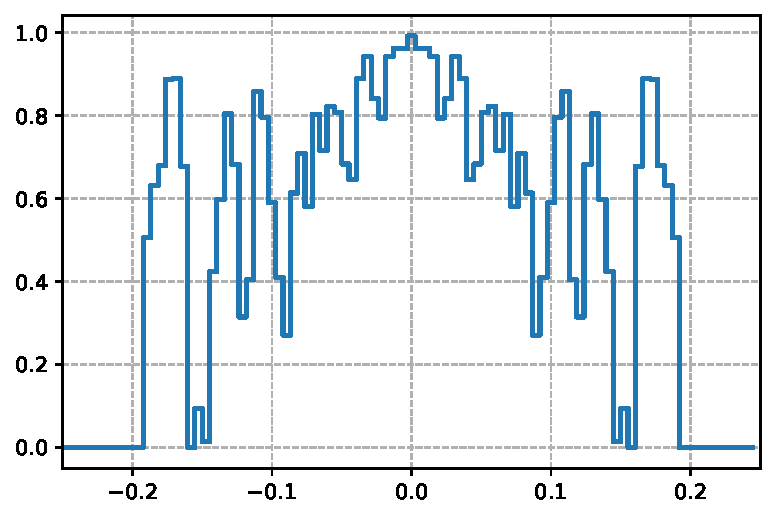
\includegraphics[scale=0.5]{figures/erdos_min_overlap.pdf}
    \caption{Construction found by \method for the minimum overlap problem of Erd\H{o}s.}
    \label{fig:erdos}
\end{figure}


~

\subsection{Sums and differences of finite sets}
Let $C_6$ be the largest constant for which the following statement holds: there exist arbitrarily large finite sets of integers $A,B$ with $|A+B| \ll |A|$ and $|A-B| \gg |A+B|^{C_6}$.
(Here $A+B = \{a+b : a \in A, b \in B\}$ and $A-B = \{a-b : a \in A, b \in B\}$ denote the sumset and difference set, respectively. The notation $X \ll Y$ means that $X \le C Y$ for some constant $C$ independent of the sets $A,B$ (for sufficiently large sets $A,B$). The notation $X \gg Y$ means that $X \ge C' Y$ for some positive constant $C'$ independent of the sets $A,B$ (for sufficiently large sets $A,B$).)
\begin{equation}\label{cds}
 1.14465 \leq C_6 \leq \frac{4}{3};
\end{equation}
see \cite[Corollary 3]{gyarmati2007sums} for the 
upper bound and \cite[Theorem 1]{gyarmati2007sums} for the lower bound. The main tool for the lower bound is the following result of \citet{gyarmati2007sums}:
\begin{equation}\label{cds-lower}
 C_6 \geq 1 + \frac{\log \frac{|U-U|}{|U+U|}}{\log (2 \max (U) + 1)}
\end{equation}
for any finite set $U$ of non-negative integers containing zero satisfying $|U-U| \leq 2 \max (U) + 1$.
\method found a set $U_1$ of size 2003 improving the lower bound to $1.1479 \leq C_6$,
and another set $U_2$ of size 54265 further improving the lower bound  to 
$1.1584 \leq C_6$.

\subsection{Packing unit regular hexagons inside a regular hexagon}
Consider the problem of packing $n$ disjoint regular hexagons with unit side length into a larger regular hexagon, minimizing the side length of the outer hexagon.
For $n=11$ and $n=12$, the best known constructions use outer hexagons of side lengths $3.943$ and $4.0$, respectively \cite{geometry_collection}.
\method found packing arrangements
that improve these bounds to $3.931$ and $3.942$, respectively.
These arrangements are shown in \Cref{fig:hexagons}.

\begin{figure}
    \centering
    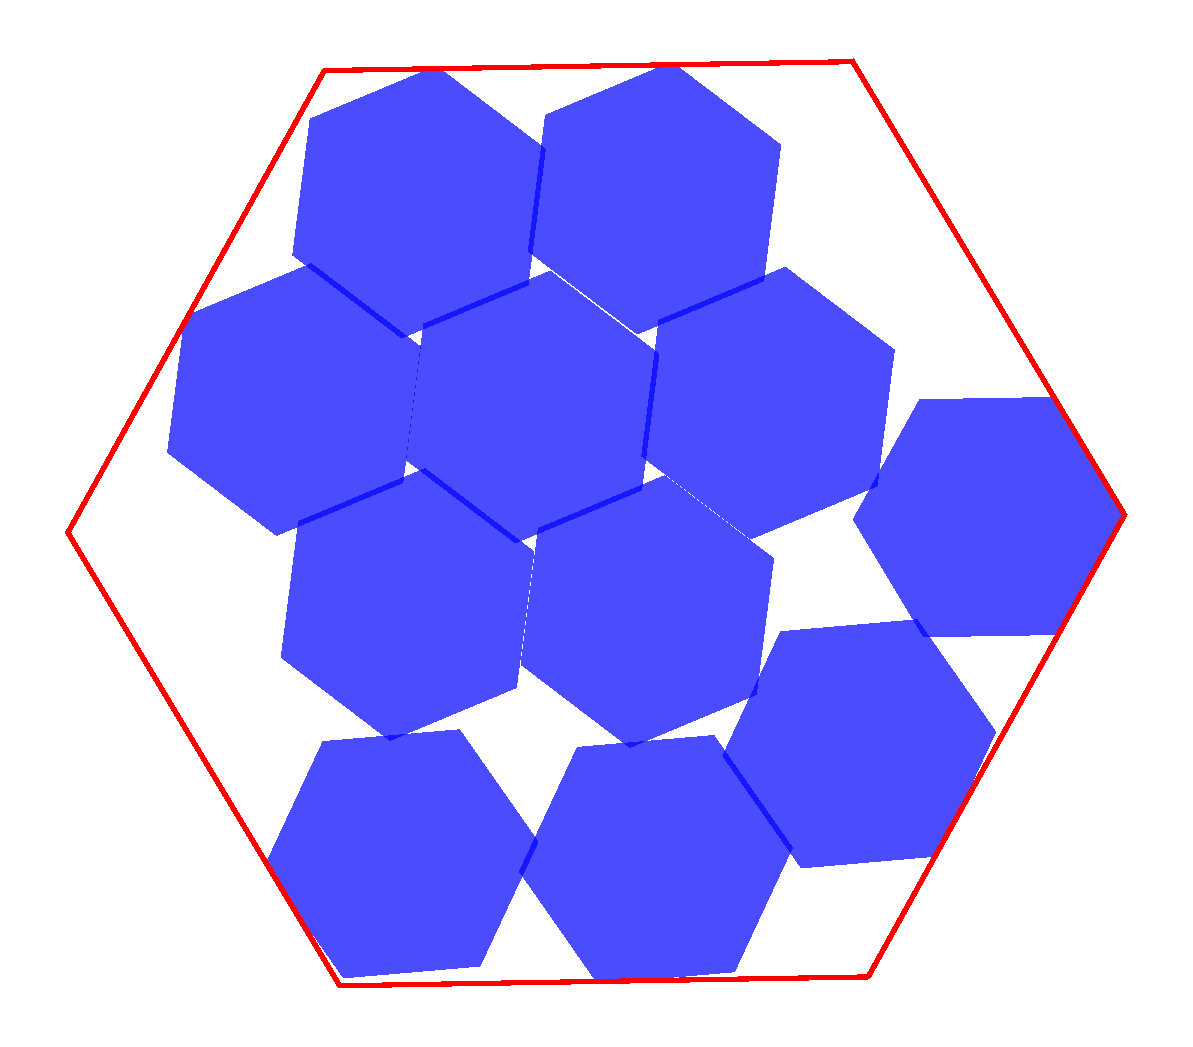
\includegraphics[width=0.4\linewidth]{figures/hexagon_11.pdf}
    \hfill
    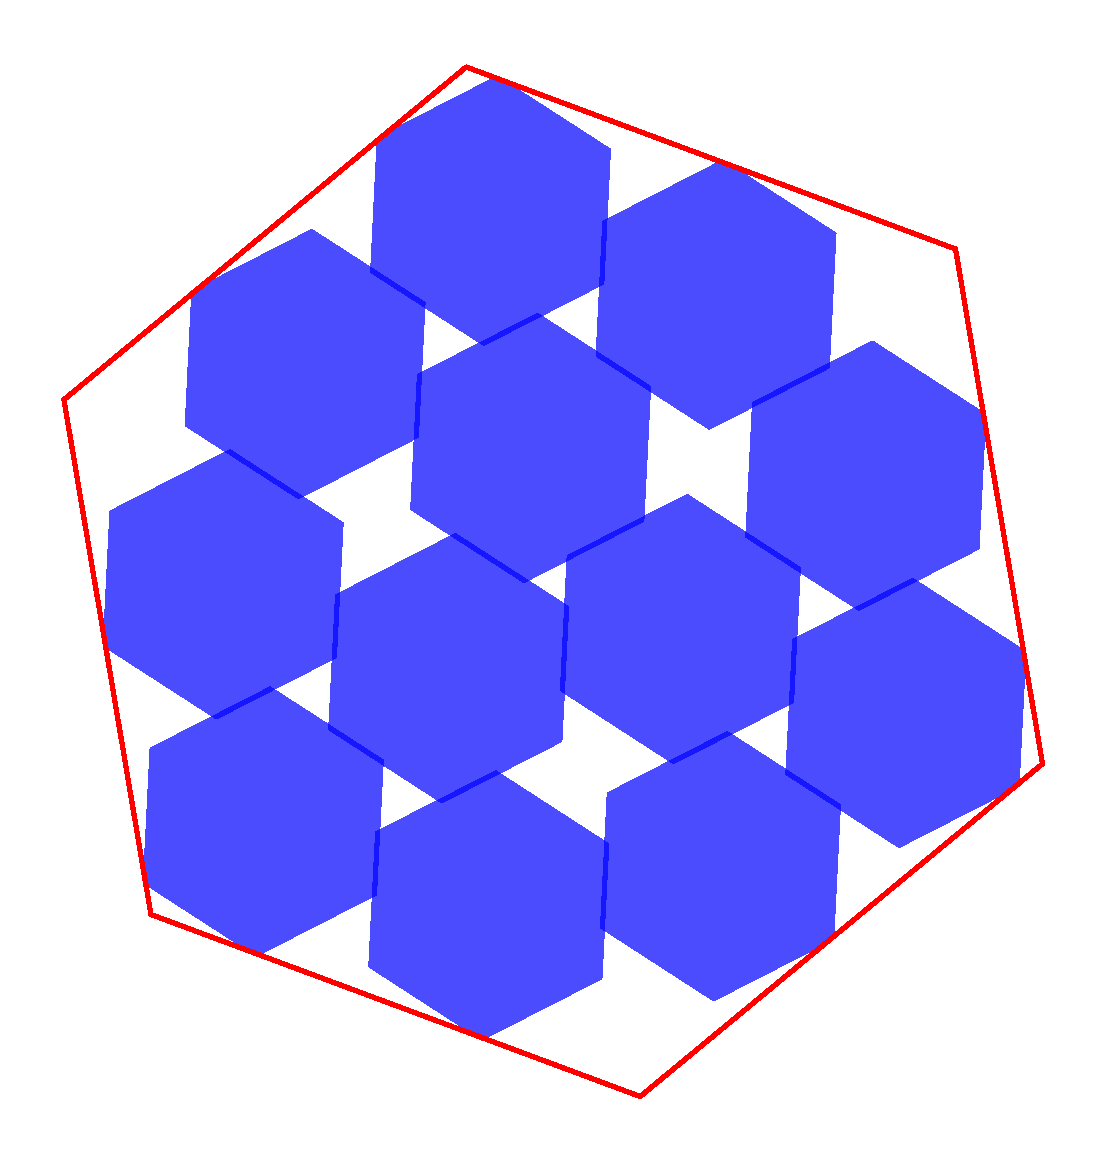
\includegraphics[width=0.4\linewidth]{figures/hexagon_12.pdf}
    \caption{Constructions of the packing problems found by \method. Left: Packing 11 unit hexagons into a regular hexagon of side length 3.931. Right: Packing 12 unit hexagons into a regular hexagon of side length 3.942.
    \label{fig:hexagons}}
\end{figure}


\subsection{Minimizing the ratio of maximum to minimum distance}
For any $n$ and $d$, the goal of this problem is to find $n$ points in the $d$-dimensional space so as to minimize the ratio between the maximum and minimum pairwise distances. \method found two new constructions improving the best known bounds.
The found constructions are shown in \Cref{fig:distance_ratios}.

In 2 dimensions, \method found 16 points with ratio $\approx \sqrt{12.889266112}$, improving the best known bound of $\sqrt{12.890}$~\citep{geometry_collection}.
(In this reference, instead of the ratio itself, the square of the ratio is reported, and we use the same convention.)
 
In 3 dimensions, \method found 14 points with ratio $\approx \sqrt{4.165849767}$, improving the best known bound of $\sqrt{4.168}$~\citep{geometry_collection}.

\begin{figure}
    \centering
    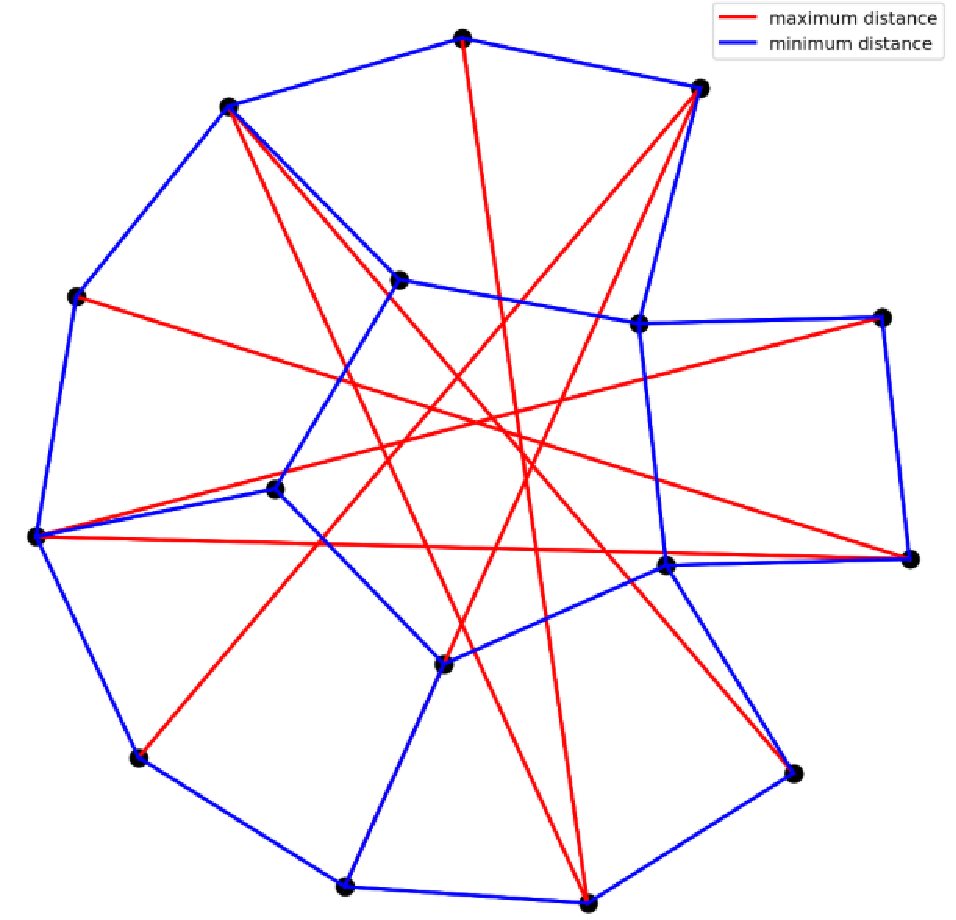
\includegraphics[width=0.45\linewidth]{figures/maxmin1.pdf}
    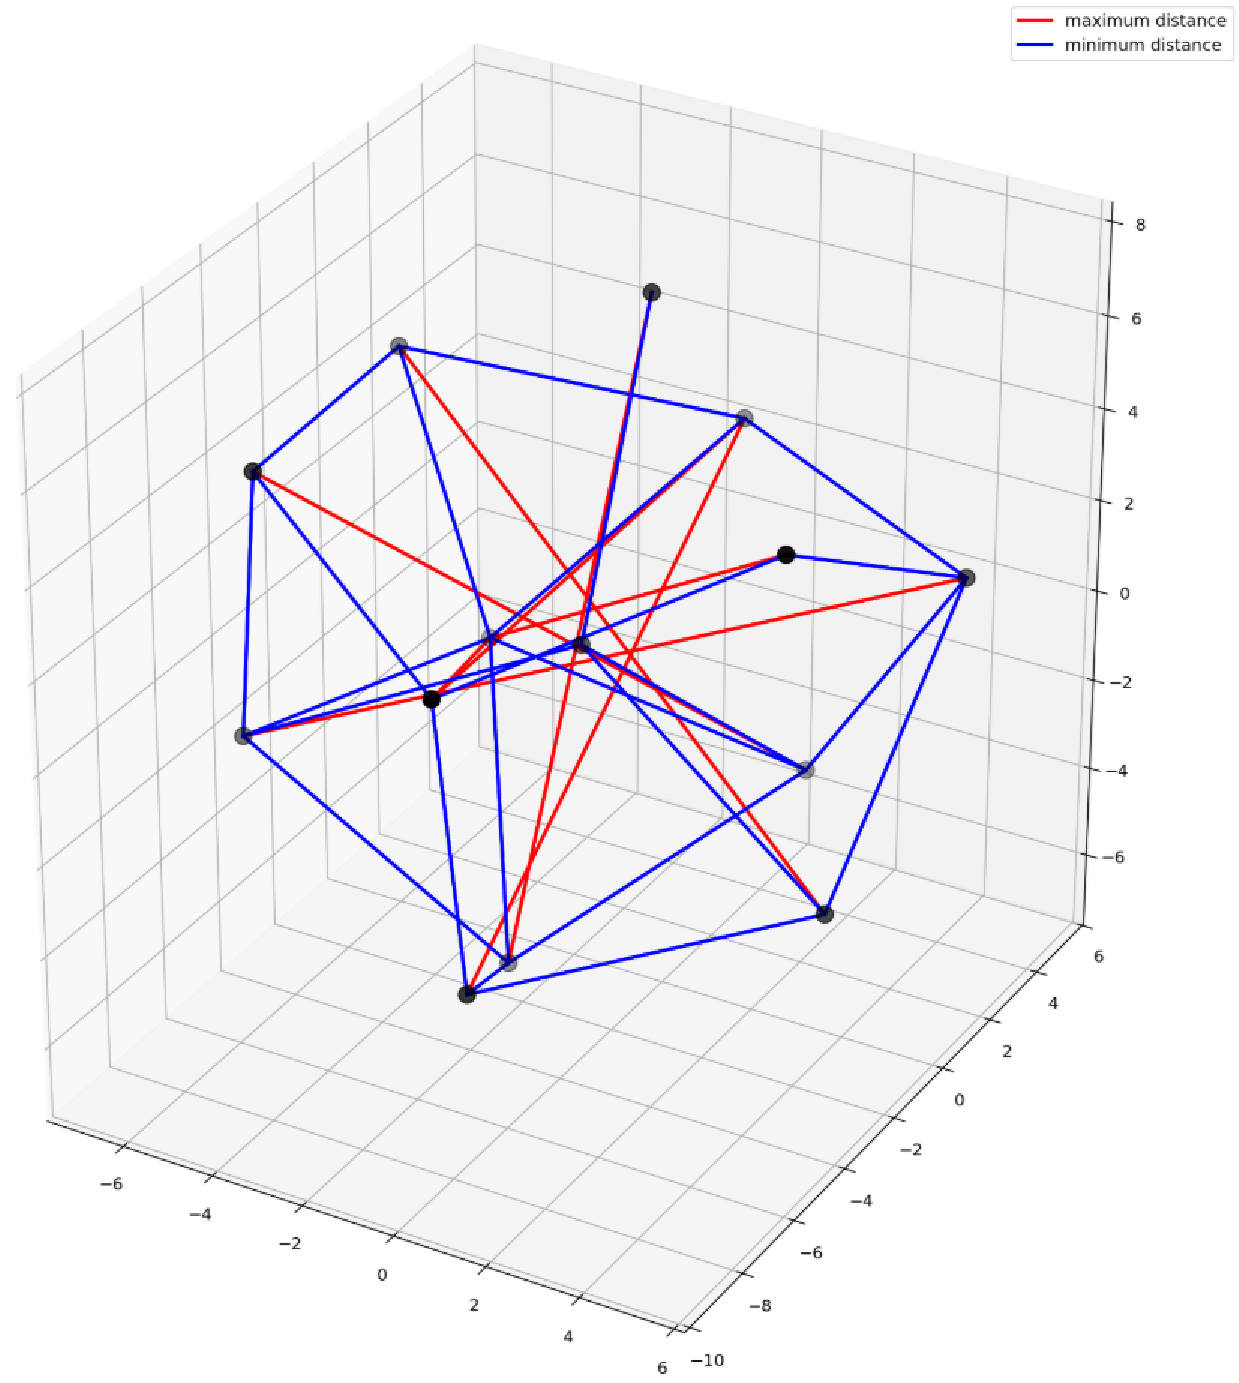
\includegraphics[width=0.45\linewidth]{figures/maxmin2.pdf}
    \caption{Left: 16 points in 2 dimensions achieving a ratio of maximum distance to minimum distance of
    $\approx \sqrt{12.889266112}$.     
    Right: 14 points in 3 dimensions achieving a ratio of $\approx \sqrt{4.165849767}$. Both constructions improve the best known bounds.}
    \label{fig:distance_ratios}
\end{figure}


\subsection{The Heilbronn problem for triangles}
The goal of this problem is to find $n$ points on or inside a triangle with unit area so that the area of the smallest triangle formed by these points is maximized. For $n=11$, the SOTA was $0.036$~\citep{geometry_collection}, and AlphaEvolve found a construction with minimum area larger than $0.0365$, which is shown in \Cref{fig:heilbronn} (left). 

\subsection{The Heilbronn problem for convex regions}
The goal of this problem is to find $n$ points on or inside a convex region with unit area so that the area of the smallest triangle formed by these points is maximized. \method improved two of the best known bounds.

For $n=13$, the SOTA was $0.0306$~\citep{geometry_collection}, and \method improved it to $0.0309$ (see \Cref{fig:heilbronn} (middle)).
For $n=14$, the SOTA was $0.0277$~\citep{geometry_collection} and \method improved it to $0.0278$ (see \Cref{fig:heilbronn} (right)).

\begin{figure}
    \centering
    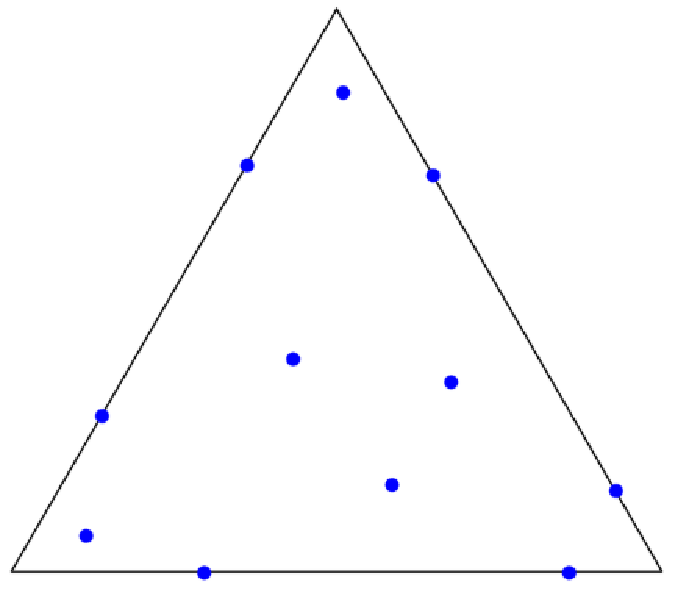
\includegraphics[width=0.25\linewidth]{figures/Heilbronn_triangle.pdf}
    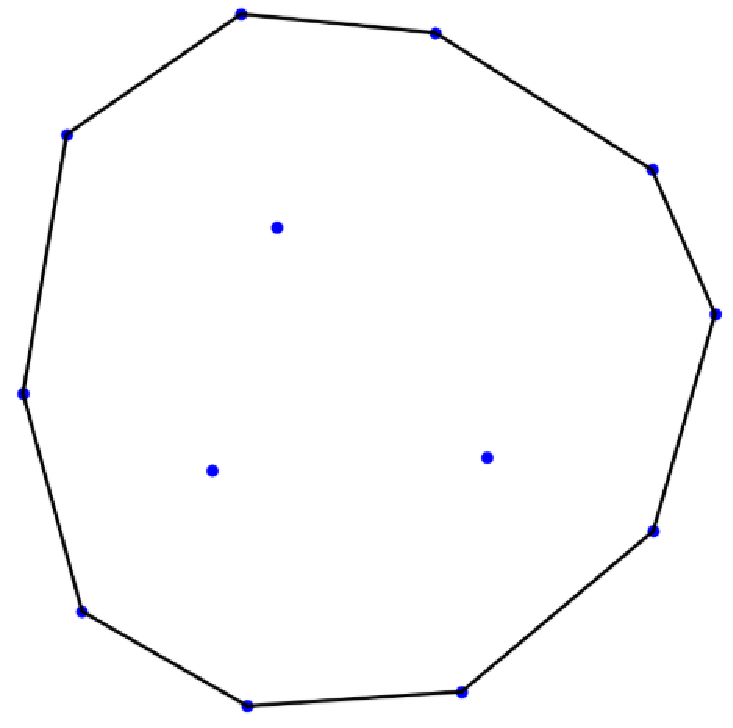
\includegraphics[width=0.25\linewidth]{figures/Heilbronn_convex_1.pdf}
    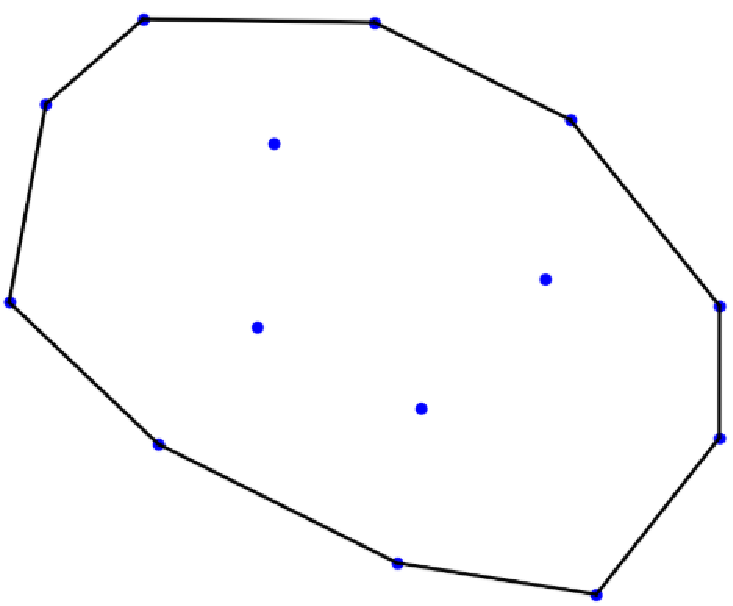
\includegraphics[width=0.25\linewidth]{figures/Heilbronn_convex_2.pdf}
    \caption{New constructions found by \method improving the best known bounds on two variants of the Heilbronn problem. Left: 11 points in a unit-area triangle with all formed triangles having area $\geq 0.0365$. Middle: 13 points inside a convex region with unit area with all formed triangles having area $\geq 0.0309$. Right: 14 points inside a unit convex region with minimum area  $\ge 0.0278$.}
    \label{fig:heilbronn}
\end{figure}


\subsection{Kissing number in dimension 11}
The kissing problem asks how many disjoint unit spheres can be packed tangent to a given unit sphere. The maximum such number in $d$ dimensions is called the \emph{$d$-dimensional kissing number~\citep{kissing_survey}}.
For $d=11$, the best known lower bound was 592~\citep{kissing_11} and \method improved this to 593. To prove the lower bound of 593 for the kissing number in dimension 11, \method found 593 many 11-dimensional non-zero points with integral coordinates such that  
the maximum norm of these points is smaller than their minimum pairwise distance.
By the following lemma, this implies the kissing number in dimension 11 is at least 593.

\begin{lemma}
Let $C \subset \mathbb{R}^d$ be a set of points satisfying
$0 \notin C$ and 
\begin{equation*}
    \min \left\{ \|x-y\| : x \neq y \in C \right\} \ge \max \left\{ \|x\|: x \in C \right\}.
\end{equation*}
Then unit spheres centred at $\left\{  \frac{2x}{\|x\|}:{x\in C}\right\}$ form a valid kissing configuration in dimension $d$. In particular, the kissing number in dimension $d$ is at least $|C|$.
\end{lemma}

\begin{proof}
For any $x\neq y \in C$, the inequality $\|x - y\|^2 \geq \max \{\|x\|^2, \|y\|^2\}$ implies
\begin{equation}
2 \langle x, y \rangle \leq \|x\|^2 + \|y\|^2 - \max \{\|x\|^2, \|y\|^2\} = \min \{\|x\|^2, \|y\|^2\} \leq \|x\|\cdot\|y\|,
\label{eq:abi}
\end{equation}
where the last inequality holds because the minimum of two positive numbers is less than or equal to their geometric mean.
The points $\left\{ \frac{2x}{\|x\|}:{x\in C}\right\}$ have norm 2, so unit spheres centred at them are tangent to a unit sphere centred at the origin.
The last step is to show that these spheres do not overlap. This is equivalent to showing, for all $x\neq y \in C$, that
\[
\left\| \frac{2x}{\|x\|} -  \frac{2y}{\|y\|}\right\| \geq 2.
\]
After simplifying, this is equivalent to
\(
2 \langle x, y \rangle  \leq \|x\|\cdot\|y\|\),
which we have proved in \eqref{eq:abi}.
Thus unit spheres centred at $\left\{ \frac{2x}{\|x\|}:{x\in C}\right\}$ form a valid kissing configuration in dimension $d$, as required.
\end{proof}


\subsection{Packing circles inside a unit square to maximize sum of radii}

Given a positive integer $n$, the problem is to pack $n$ disjoint circles inside a unit square so as to maximize the sum of their radii. \method found two new constructions improving the state of the art~\citep{geometry_collection}.

For $n=26$, the SOTA was $2.634$, and AlphaEvolve improved it to $2.635$; see \Cref{fig:circle_packing} (left).
For $n=32$, the SOTA was $2.936$, and AlphaEvolve improved it to $2.937$; see \Cref{fig:circle_packing} (middle).

\subsection{Packing  circles inside a rectangle of perimeter 4 to maximize sum of radii}
Given a positive integer $n$, the problem is to pack $n$ disjoint circles inside a rectangle of perimeter 4 so as to maximize the sum of their radii. 
\method found a new construction for $n=21$, improving the state of the art from $2.364$~\citep{geometry_collection} to $2.3658$; see \Cref{fig:circle_packing} (right).

\begin{figure}[b]
    \centering
    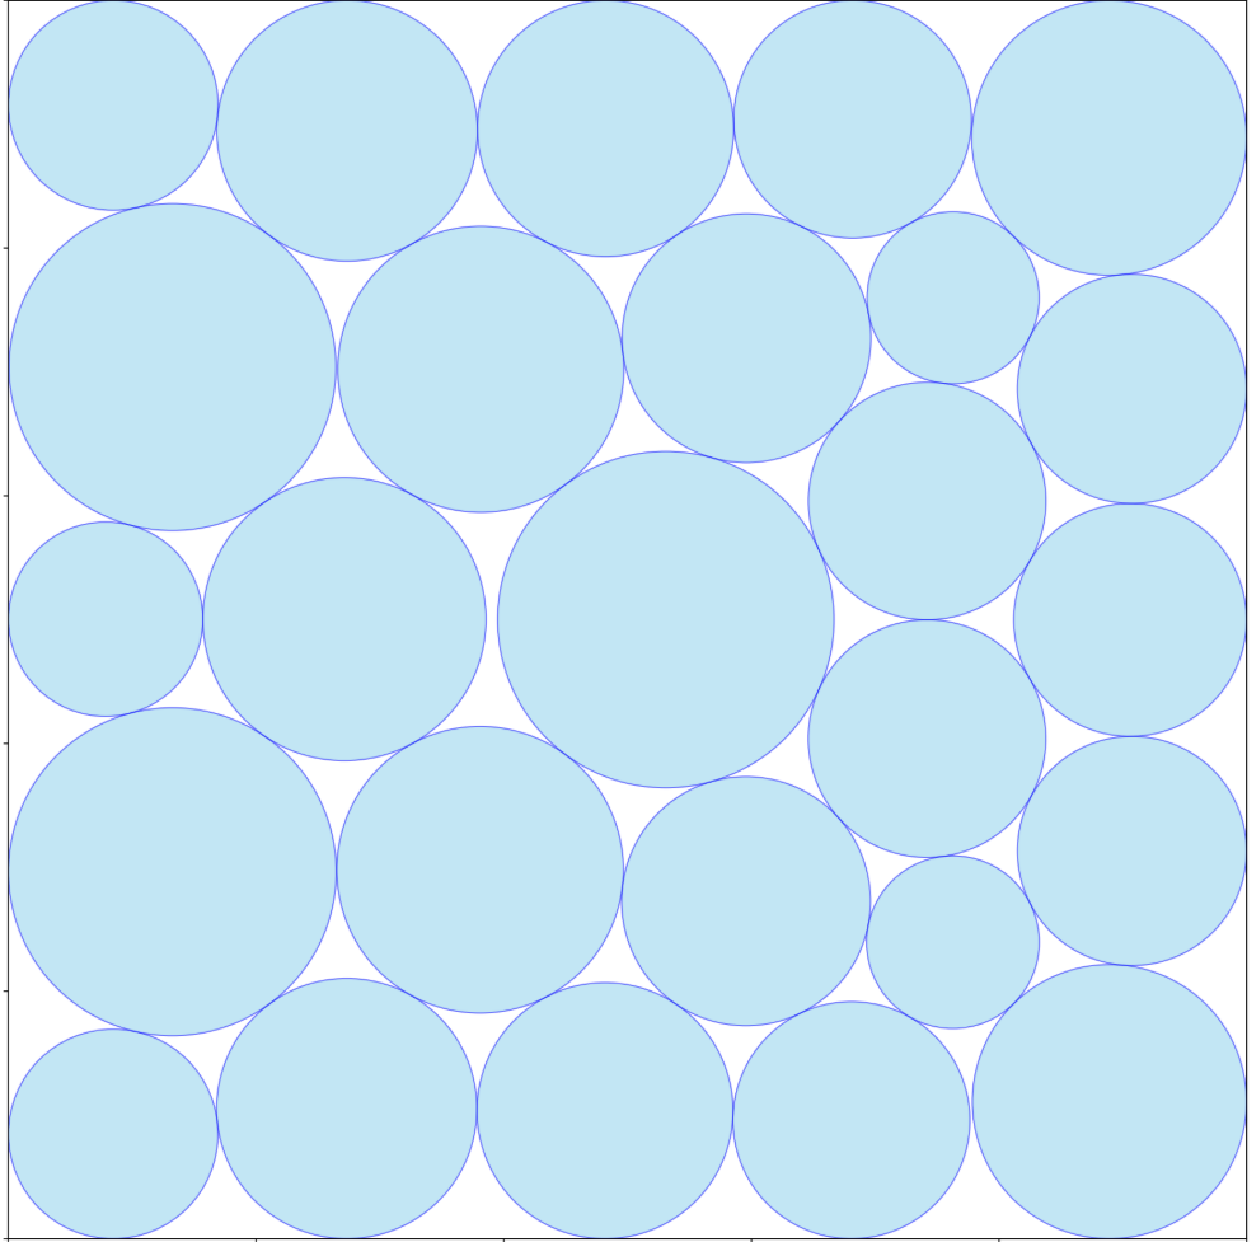
\includegraphics[width=0.25\linewidth]{figures/circles_1.pdf}
    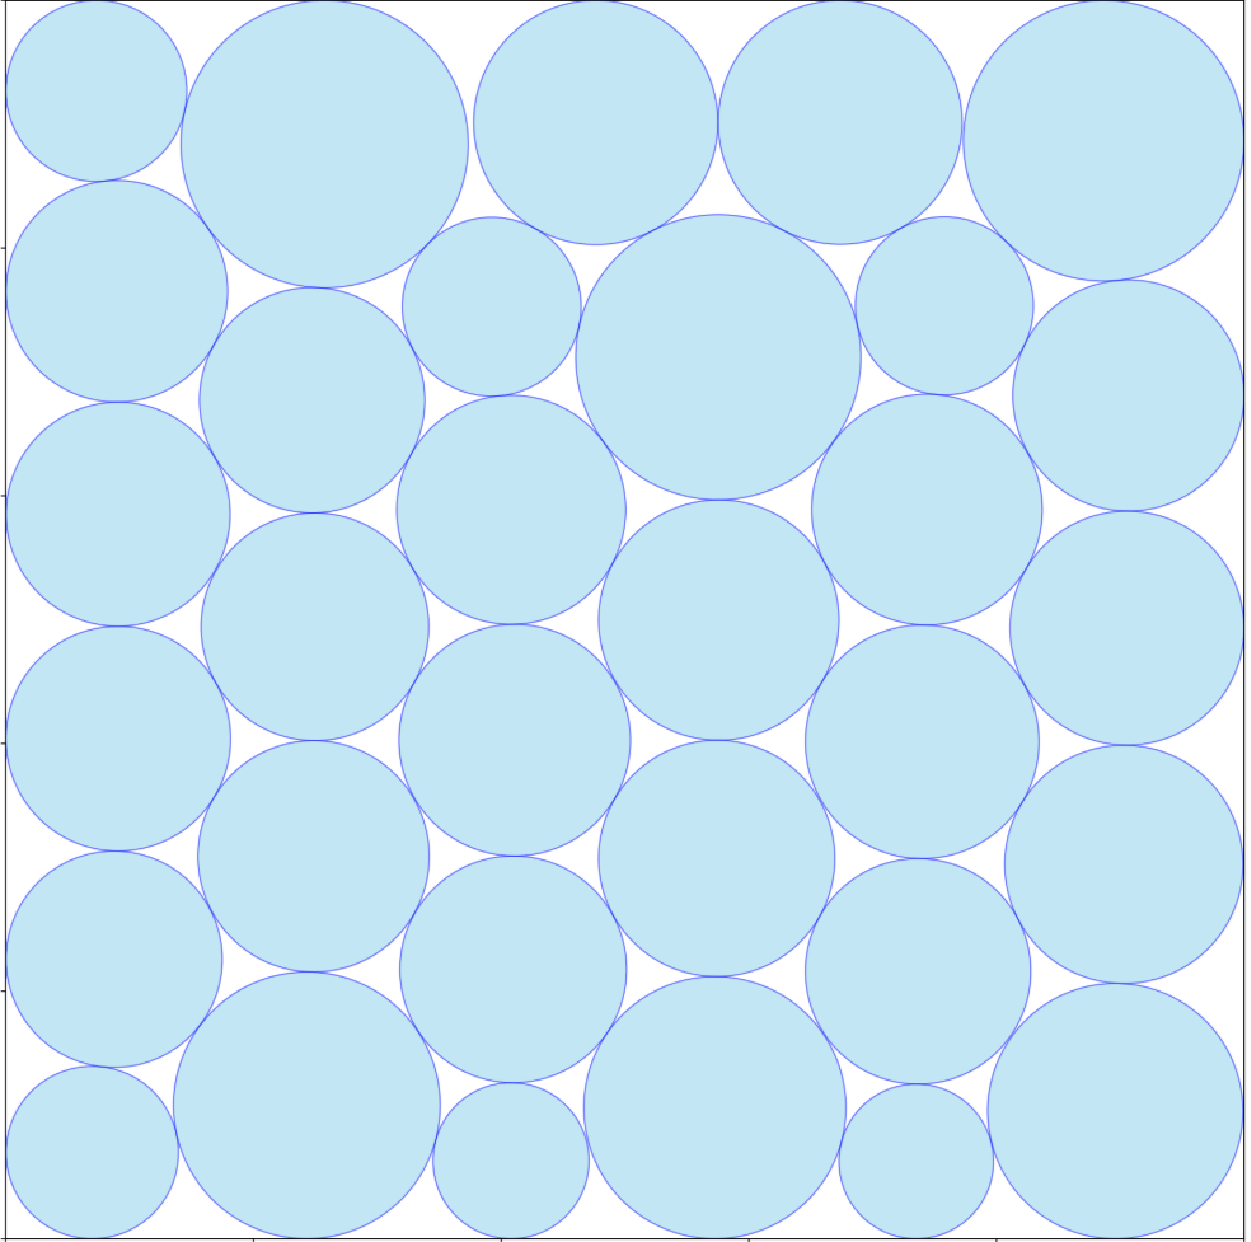
\includegraphics[width=0.25\linewidth]{figures/circles_2.pdf}
    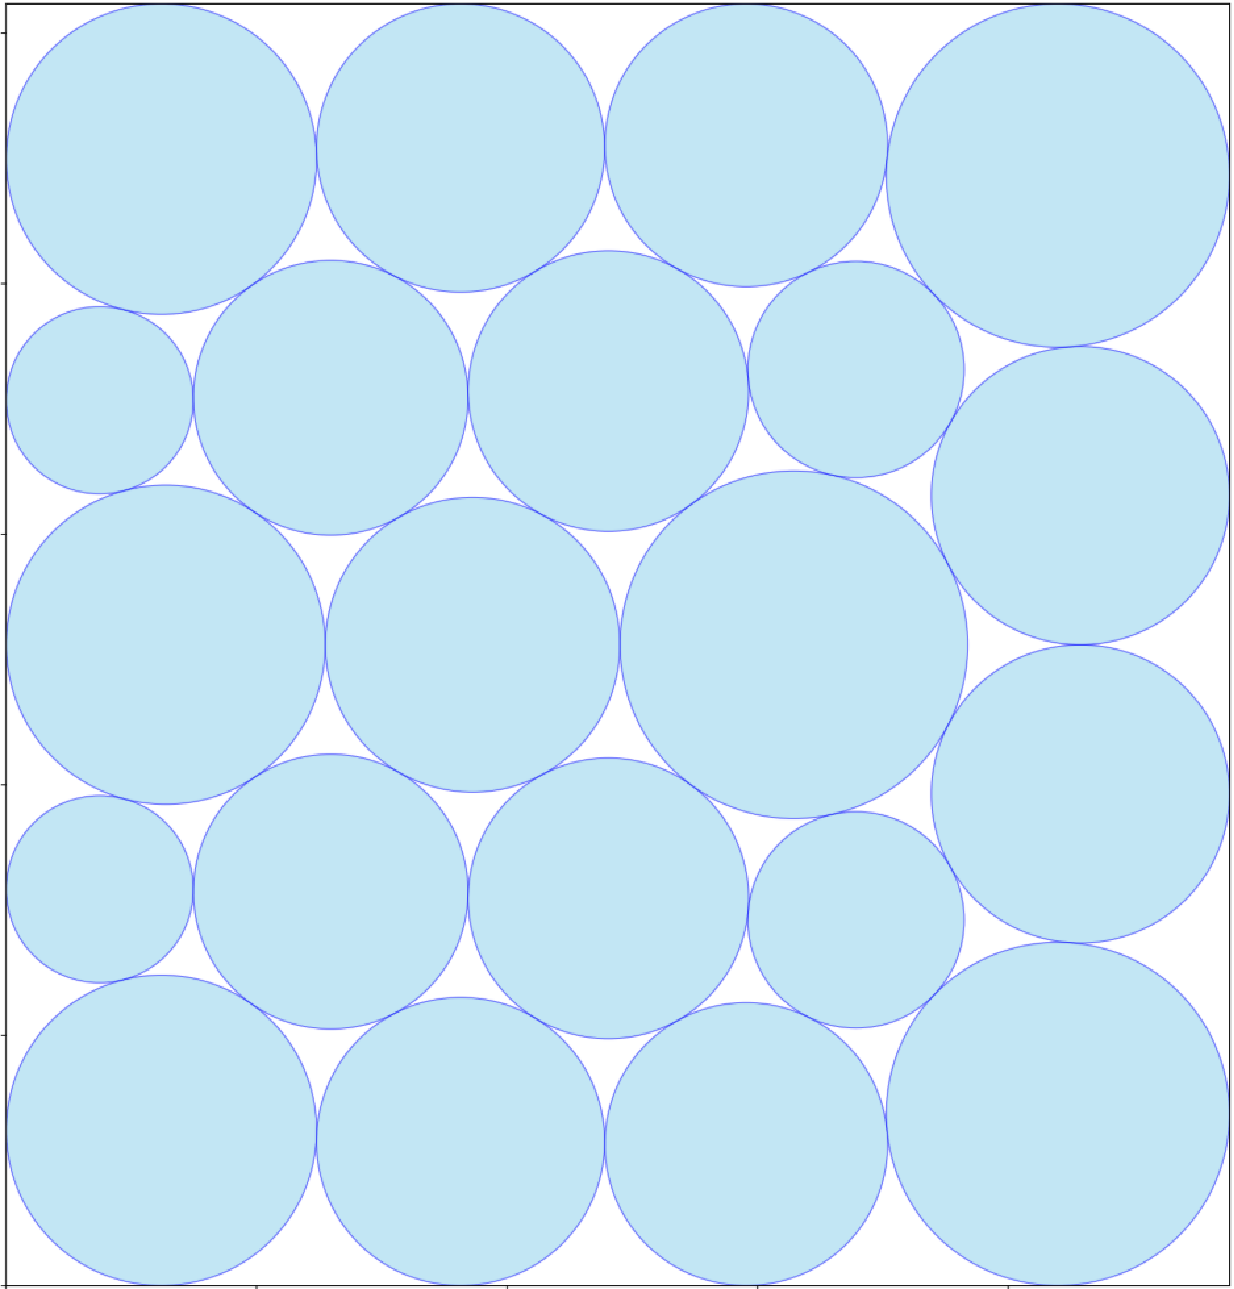
\includegraphics[width=0.25\linewidth]{figures/circles_3.pdf}
    \caption{New constructions found by \method improving the best known bounds on packing circles to maximize their sum of radii. Left: $26$ circles in a unit square with sum of radii $\geq 2.635$. Middle: $32$ circles in a unit square with sum of radii $\geq 2.937$. Right: 21 circles in a rectangle with perimeter $4$, with sum of radii $\geq 2.365$.}
    \label{fig:circle_packing}
\end{figure}
